\documentclass{article}

\usepackage{amsmath}
\usepackage{amssymb}
\usepackage{parskip}
\usepackage{fullpage}
\usepackage{hyperref}
\usepackage{wrapfig}
\usepackage{tikz}

\hypersetup{
    colorlinks=true,
    linkcolor=black,
    urlcolor=blue,
    pdftitle={ComplexAnalysis},
    pdfpagemode=FullScreen,
}

\usetikzlibrary{3d,arrows.meta,decorations.markings,perspective}
\tikzset{->-/.style={decoration={% https://tex.stackexchange.com/a/39282/194703
  markings,
  mark=at position #1 with {\arrow{>}}},postaction={decorate}},
  ->-/.default=0.55}

\title{Complex Analysis}
\author{Paolo Bettelini}
\date{}

\begin{document}

\maketitle
\tableofcontents
\pagebreak

\section{De Moivre's Theorem}

Using the property of exponentiation \(\left(a^b\right)^c = a^{bc}\),
we can see that \(\left(e^{i\theta}\right)^n = e^{in\theta}\).
\\
Using Euler's formula we can deduce that

\[
    \left(\cos(\theta) + i\sin(\theta)\right)^n = \cos(n\theta) + i\sin(n\theta),
	\quad n \in \mathbb{Z}
\]

\section{Nth Roots of Units}

We can extend De Moivre's Theorem for the integers powers or any complex number,
rather than the ones on the unit circle \((r=1)\).

\[
    \left(r\left(\cos(\theta) + i\sin(\theta)\right)\right)^n = 
	r^n\left(\cos(n\theta) + i\sin(n\theta)\right), \quad n \in \mathbb{Z}
\]

The nth roots of \(1\) are the solutions to

\[
	x^n=1
\]

for a given \(n\). We might write \(1\) as a complex number

\[
	x^n = \cos(0) + i\sin(0)
\]

Comparing this to our extended De Moivre's theorem

\[
	\cos(0) + i\sin(0) = r^n\left(\cos(n\theta) + i\sin(n\theta)\right)
\]

We can see that

\begin{align*}
	r^n&=1 \\
	n\theta&=0
\end{align*}

As long as \(n \neq 0\)

\begin{align*}
	r&=1 \\
	\theta&=0
\end{align*}

By plugging these values into

\[
	x^n = \left(r\left(\cos(\theta) + i\sin(\theta)\right)\right)^n
\]

we get that \(x=1\).

However we could also write \(1\) as

\[
	\cos(2k\pi) + i\sin(2k\pi), \quad k\in \mathbb{Z}
\]

We would then get that

\begin{align*}
	r^n&=1 \\
	n\theta&=2k\pi
\end{align*}

When solving for \(x\) again we get

\begin{align*}
	x^n &= \left(r\left(\cos(\theta) + i\sin(\theta)\right)\right)^n
	\\
	&= \left(\cos\left(\frac{2k\pi}{n}\right) + i\sin\left(\frac{2k\pi}{n}\right)\right)^n
\end{align*}

concluding that

\[
	x = \cos\left(\frac{2k\pi}{n}\right) + i\sin\left(\frac{2k\pi}{n}\right)
\]

This gives us a solution for each \(k\), however the solutions are redundant for \(k \geq n\).
In fact, the roots of unity of \(n\) are \(n\) distinct solutions (points on the unit circle).

\def\n{7}
\begin{wrapfigure}[4]{l}{4.5cm} % 4 is the number of wrapfigure lines
\begin{tikzpicture}[
        dot/.style={draw,fill,circle,inner sep=1pt}
    ]
    \draw[->] (-2,0) -- (2,0) node[below] {\(\Re\)};
    \draw[->] (0,-2) -- (0,2) node[left] {\(\Im\)};
    \draw[help lines] (0,0) circle (1);
    
    \foreach \i in {1,...,\n} {
        \node[dot,label={\i*360/\n-(\i==\n)*45:\(\zeta_\n^{\i}\)}] (w\i) at (\i*360/\n:1) {};
        \draw[->] (0,0) -- (w\i);
    }
    \draw[->] (0:.3) arc (0:360/\n:.3);
    \node at (360/\n/2:.5) {\(\alpha\)};
\end{tikzpicture}
\end{wrapfigure}

\phantom{ }\\
    
The roots of units have the same angle \(\alpha = \frac{2\pi}{n}\) between eachother.
\\
The first root of unit counter-clockwise is denoted \(\zeta_n\) because each subsequent
root is a power of \(\zeta_n\). In this case, \(\zeta_\n\).

\pagebreak

\section{Riemann Spheres}

A Riemann sphere is a unit sphere used to represent the complex plane
using stereographic projection.

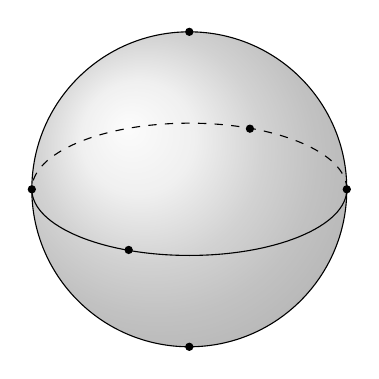
\begin{tikzpicture}[scale=2]
    \shade[ball color = gray!40, opacity = 0.4] (0,0) circle (1cm);
    \draw (0,0) circle (1cm);

    \draw (-1,0) arc (180:360:1 and 0.42);
    \draw[dashed] (1,0) arc (0:180:1 and 0.42);

    %\draw (0,-1) arc (180:180:1 and 0.42);
    % \draw[dashed] (0,1) arc (90:270:1 and 0.42);
    
    \fill[fill=black] (0,0,-1) circle (0.75pt);
    \fill[fill=black] (0,0,1) circle (0.75pt);
    \fill[fill=black] (0,1,0) circle (0.75pt);
    \fill[fill=black] (0,-1,0) circle (0.75pt);
    \fill[fill=black] (1,0,0) circle (0.75pt);
    \fill[fill=black] (-1,0,0) circle (0.75pt);
    %\filldraw[
    %    draw=red,%
    %    fill=red!20,%
    %]          (0,0,0)
    %        -- (\x,{sqrt(3)*\x},0)
    %        -- (\x,{sqrt(3)*\x},1)
    %        -- (0,0,1)
    %        -- cycle;
  \end{tikzpicture}

The Riemann sphere lays on the complex plane. A complex number
is represented by the intersection between the sphere
and a ray starting from the topmost point of the sphere
and intersecting with the given complex number on the complex plane.

\end{document}
